% Chapter Template

\chapter{Results} % Main chapter title

\label{Chapter8} % Change X to a consecutive number; for referencing this chapter elsewhere, use \ref{ChapterX}

\lhead{Chapter 8. \emph{Results}} % Change X to a consecutive number; this is for the header on each page - perhaps a shortened title

%----------------------------------------------------------------------------------------
%	SECTION 1
%----------------------------------------------------------------------------------------

\section{Experimental Setting and Results}

The application is tested for the following experimental setup. Since the proposed application aim to be used in the hospital, thus there are only specific sheets of cloth to be tested. Each experiment uses twenty tested image. The experiment setups are classified as shown in Figure \ref{fig:f801}.

Conditions testing of sheets of cloth are separated following color. There are green color, white color and both colors. In each color of sheets of cloth includes vertical axis and horizontal axis. In each vertical axis and horizontal axis includes four cases. The cases is shown in Table \ref{tab:t801}. After the conditions are specified, the application experimental will be begun.
\begin{figure}[t]
	\centering
	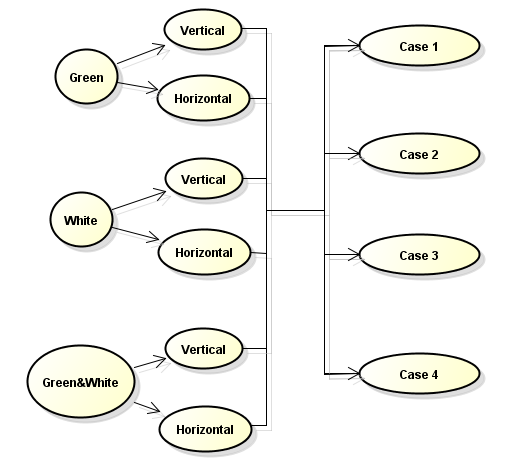
\includegraphics[scale=0.7]{f801.png}
	\caption{Conditions testing}
	\label{fig:f801}
\end{figure}
\begin{table}[t]
	\centering
	\begin{tabular}{|l|l|l|l|l|l|l|}
		\hline
		Case & Direction & Top-Boarder & Lower-Boarder & Direction & Left-Boarder & Right- Boarder\\
		\hline
		1 & Horizontal & Cloth & Cloth & Vertical & Cloth & Cloth\\
		\hline
		2 & Horizontal & Cloth & Not Cloth & Vertical & Cloth & Not Cloth\\
		\hline
		3 & Horizontal & Not Cloth & Cloth & Vertical & Not Cloth & Cloth\\
		\hline
		4 & Horizontal & Not Cloth & Not Cloth & Vertical & Not Cloth & Not Cloth\\
		\hline
	\end{tabular}
	\caption{Cases testing}
	\label{tab:t801}
\end{table}

Green color testing\\
test 1: number of sheets of cloth is fixed at ten in vertical axis.\\ 
test 2: number of sheets of cloth is fixed at ten in horizontal axis.\\
test 3: number of sheets of cloth is not fixed at ten in vertical axis.\\ 
test 4: number of sheets of cloth is not fixed at ten in horizontal axis.\\
%----------------------------
%--Test 1
%---------------------------
\begin{table}[t]
	\centering
	\begin{tabular}{|p{1.5cm}|p{1.5cm}|p{1.5cm}|p{1.5cm}|p{1.5cm}|}
		\hline
		& Case 1 & Case 2 & Case 3 & Case 4\\
		\hline
		Actual Number & Counting Number & Counting Number & Counting Number & Counting Number\\
		\hline
		10 	& 10	& 8 & 8 	& 9	\\
		10  & 8	 	& 9 & 8		& 9	\\
		10	& 8		& 8	& 10	& 9	\\
		10	& 9		& 9	& 8		& 8	\\
		10	& 9		& 9	& 9		& 9	\\
		total(\%)& 	88	& 86	&	86	& 88	\\
		\hline
	\end{tabular}
	\caption{Test 1} \label{teb:test801}
\end{table}
%----------------------------
%--Test 2
%---------------------------
\begin{table}[t]
	\centering
	\begin{tabular}{|p{1.5cm}|p{1.5cm}|p{1.5cm}|p{1.5cm}|p{1.5cm}|}
		\hline
		& Case 1 & Case 2 & Case 3 & Case 4\\
		\hline
		Actual Number & Counting Number & Counting Number & Counting Number & Counting Number\\
		\hline
		 10	&   10	&  	9	&  	7	& 10	\\
		 10	& 	10 	& 	9	& 	9	& 10	\\
		10	& 	9	&	9	& 	7	& 9	\\
		10	& 	10	& 	9	& 	6	& 9	\\
		10	& 	9	& 	9	& 	7	& 8	\\
		total( \%)& 96		&	90	&	72	& 92	\\
		\hline
	\end{tabular}
	\caption{Test 2} \label{teb:test802}
\end{table}
%----------------------------
%--Test 3
%---------------------------
\begin{table}[t]
	\centering
	\begin{tabular}{|p{1.5cm}|p{1.5cm}|p{1.5cm}|p{1.5cm}|p{1.5cm}|}
		\hline
		& Case 1 & Case 2 & Case 3 & Case 4\\
		\hline
		Actual Number & Counting Number & Counting Number & Counting Number & Counting Number\\
		\hline
	5	& 	5	&  	5	&  	5	& 5		\\
	10	& 	10 	& 	10	& 	9	& 9		\\
	15	& 	13	&	12	& 	14	& 12	\\
	20	& 	19	& 	16	& 	17	& 18	\\
	25	& 	23	& 	21	& 	22	& 20	\\
		total(\%)& 	93.33	&	85.33	&	89.33	& 85.33	\\
		\hline
	\end{tabular}
	\caption{Test 3} \label{teb:test803}
\end{table}
%----------------------------
%--Test 4
%---------------------------
\begin{table}[t]
	\centering
	\begin{tabular}{|p{1.5cm}|p{1.5cm}|p{1.5cm}|p{1.5cm}|p{1.5cm}|}
		\hline
		& Case 1 & Case 2 & Case 3 & Case 4\\
		\hline
		Actual Number & Counting Number & Counting Number & Counting Number & Counting Number\\
		\hline
	5	& 	5	&  5	&  	5	& 5	\\
	10	& 	10	& 	10	& 	11	& 7	\\
	15	& 	14	&	12	& 	14	& 10	\\
	20	& 	17	& 	15	& 	12	& 14	\\
	25	& 	22	& 	15	& 	15	& 17	\\
		total(\%)& 	90.67	&	76	&	76	& 70.67	\\
		\hline
	\end{tabular}
	\caption{Test 4} \label{teb:test804}
\end{table}

White color testing\\
test 5: number of sheets of cloth is fixed at ten in vertical axis.\\ 
test 6: number of sheets of cloth is fixed at ten in horizontal axis.\\ 
test 7: number of sheets of cloth is not fixed at ten in vertical axis.\\ 
test 8: number of sheets of cloth is not fixed at ten in horizontal axis.\\
%----------------------------
%--Test 5
%---------------------------
\begin{table}[t]
	\centering
	\begin{tabular}{|p{1.5cm}|p{1.5cm}|p{1.5cm}|p{1.5cm}|p{1.5cm}|}
		\hline
		& Case 1 & Case 2 & Case 3 & Case 4\\
		\hline
		Actual Number & Counting Number & Counting Number & Counting Number & Counting Number\\
		\hline
	10	& 	8	&  	7	&  	7	& 8	\\
	10	& 	 8	& 	7	& 	7	& 8	\\
	10	& 	9	&	5	& 	8	& 6	\\
	10	& 	8	& 	8	& 	8	& 7	\\
	10	& 	8	& 	9	& 	7	& 9	\\
		total(\%)& 	82	&	72	&	74	& 76	\\
		\hline
	\end{tabular}
	\caption{Test 5} \label{teb:test805}
\end{table}
%----------------------------
%--Test 6
%---------------------------
\begin{table}[t]
	\centering
	\begin{tabular}{|p{1.5cm}|p{1.5cm}|p{1.5cm}|p{1.5cm}|p{1.5cm}|}
		\hline
		& Case 1 & Case 2 & Case 3 & Case 4\\
		\hline
		Actual Number & Counting Number & Counting Number & Counting Number & Counting Number\\
		\hline
	10	& 	10	&  10	&  	7	& 10	\\
	10	& 	 10	& 	10	& 	9	& 10	\\
	10	& 	10	&	9	& 	7	& 9	\\
	10	& 	9	& 	9	& 	6	& 9	\\
	10	& 	9	& 	9	& 	7	& 8	\\
		total(\%)& 	96	&	94	&	72	& 92\\
		\hline
	\end{tabular}
	\caption{Test 6} \label{teb:test806}
\end{table}
%----------------------------
%--Test 7
%---------------------------
\begin{table}[t]
	\centering
	\begin{tabular}{|p{1.5cm}|p{1.5cm}|p{1.5cm}|p{1.5cm}|p{1.5cm}|}
		\hline
		& Case 1 & Case 2 & Case 3 & Case 4\\
		\hline
		Actual Number & Counting Number & Counting Number & Counting Number & Counting Number\\
		\hline
	8	& 	6	&  	7	&  	5	& 7	\\
	11	& 	 9	& 	9	& 	9	& 9	\\
	12	& 	11	&	11	& 	11	& 12	\\
	15	& 	11	& 	11	& 	12	& 12\\
	20	& 	13	& 	13	& 	13	& 12	\\
		total(\%)& 	75.75	&	77.72	&	75.75	& 78.78\\
		\hline
	\end{tabular}
	\caption{Test 7} \label{teb:test807}
\end{table}
%----------------------------
%--Test 8
%---------------------------
\begin{table}[t]
	\centering
	\begin{tabular}{|p{1.5cm}|p{1.5cm}|p{1.5cm}|p{1.5cm}|p{1.5cm}|}
		\hline
		& Case 1 & Case 2 & Case 3 & Case 4\\
		\hline
		Actual Number & Counting Number & Counting Number & Counting Number & Counting Number\\
		\hline
	8	& 	7	&  	8	&  	7	& 8	\\
	12	& 	 10	& 	10	& 	10	& 10	\\
	15	& 	11	&	12	& 	9	& 	13\\
	16	& 	13	& 	12	& 	10	& 	11\\
	20	& 	17	& 	16	& 	16	& 	9\\
		total(\%)& 	87.87	&	80.30	&	78.78	& 77.27 \\
		\hline
	\end{tabular}
	\caption{Test 8} \label{teb:test808}
\end{table}

Both color testing\\ 
test 9: number of sheets of cloth is fixed at ten in horizontal axis.\\  
test 10: number of sheets of cloth is not fixed at ten in horizontal axis.\\
%----------------------------
%--Test 9
%---------------------------
\begin{table}[t]
	\centering
	\begin{tabular}{|p{1.5cm}|p{1.5cm}|p{1.5cm}|p{1.5cm}|p{1.5cm}|}
		\hline
		& Case 1 & Case 2 & Case 3 & Case 4\\
		\hline
		Actual Number & Counting Number & Counting Number & Counting Number & Counting Number\\
		\hline
	10	& 	2	&  	1	&  	1	& 1	\\
	10	& 	 2	& 	2	& 	9	& 5	\\
	10	& 	4	&	5	& 	7	& 5	\\
	10	& 	4	& 	6	& 	5	& 6	\\
	10	& 	3	& 	4	& 	4	& 4	\\
		total(\%)& 	30	&	36	&	52	& 42\\
		\hline
	\end{tabular}
	\caption{Test 9} \label{teb:test809}
\end{table}
%----------------------------
%--Test 10
%---------------------------
\begin{table}[t]
	\centering
	\begin{tabular}{|p{1.5cm}|p{1.5cm}|p{1.5cm}|p{1.5cm}|p{1.5cm}|}
		\hline
		& Case 1 & Case 2 & Case 3 & Case 4\\
		\hline
		Actual Number & Counting Number & Counting Number & Counting Number & Counting Number\\
		\hline
	7	& 	2	&  	2	&  	3	& 3	\\
	9	& 	 2	& 	2	& 	6	& 4	\\
	10	& 	4	&	4	& 	4	& 4	\\
	10	& 	4	& 	2	& 	2	& 2	\\
	11	& 	6	& 	6	& 	6	& 6	\\
		total(\%)& 	38.30	&	34.04	&	44.68	& 40.43\\
		\hline
	\end{tabular}
	\caption{Test 10} \label{teb:test8010}
\end{table}

From the Experimental, the best case of green sheets of cloth is case number one. It means that the best result will be obtained when users take an image in horizontal axis sheets of clothas shown in Table \ref{teb:test801} - \ref{teb:test804}. the best case of white sheets of cloth is also case number one as shown in Table \ref{teb:test805} - \ref{teb:test808}. So sheets of cloth in horizontal axis is the best way to obtain the best result. 
 From above summarize, both color testing will be tested in only horizontal axis. So the result is shown in Table \ref{teb:test809} - \ref{teb:test8010}. 
 
 Conclusion, a good result will be obtained when color sheets of cloth was same color and directed in horizontal axis. An accurate of case number one more than 80 percent.